\entry{2026-10-08}{Mechanism: the gain is the exact gradient (A1, A2)}

Lane \texttt{2026-10-06-jcp-mechanism} (last commit \texttt{712d682d8}, mirror \texttt{977b28357}); jobs 5012942 (A1 3D), 5015576 (A1 2D), 5016189 (A2), all on H200, f64, \texttt{jax\_backend=gpu}. Every step passed a Codex gate; the final report audit had no WRONG items. Report: \path{worktrees/2026-10-06-jcp-mechanism/experiments/jcp-mechanism/report.md}. \textbf{Preliminary; accuracy against first-order references is provisional.}

\subsection*{A1: mesh nodes with the exact gradient}
A control arm keeps every mesh node but uses the bank's analytic derivative instead of the upwind stencil.
In 3D (64\textsuperscript{3}, 128\textsuperscript{3}; $R'=512, 256$; 64 validation cases) it reproduces the converged off-mesh rollout in all four cells (pre-registered label R): the old tensor's worst error is about 10\,\% (64\textsuperscript{3}) and 6\,\% (128\textsuperscript{3}), while the mesh-node arm, Gauss $24^3$ and the 32768-point lattice all sit near 3.1\,\%.
In 2D the pre-registered rule could not be applied (label X0: the dense-vs-converged gap was below the 1\,\% threshold), but descriptively the mesh-node arm is again far closer to the converged rollout than the dense stencil solve.
\begin{center}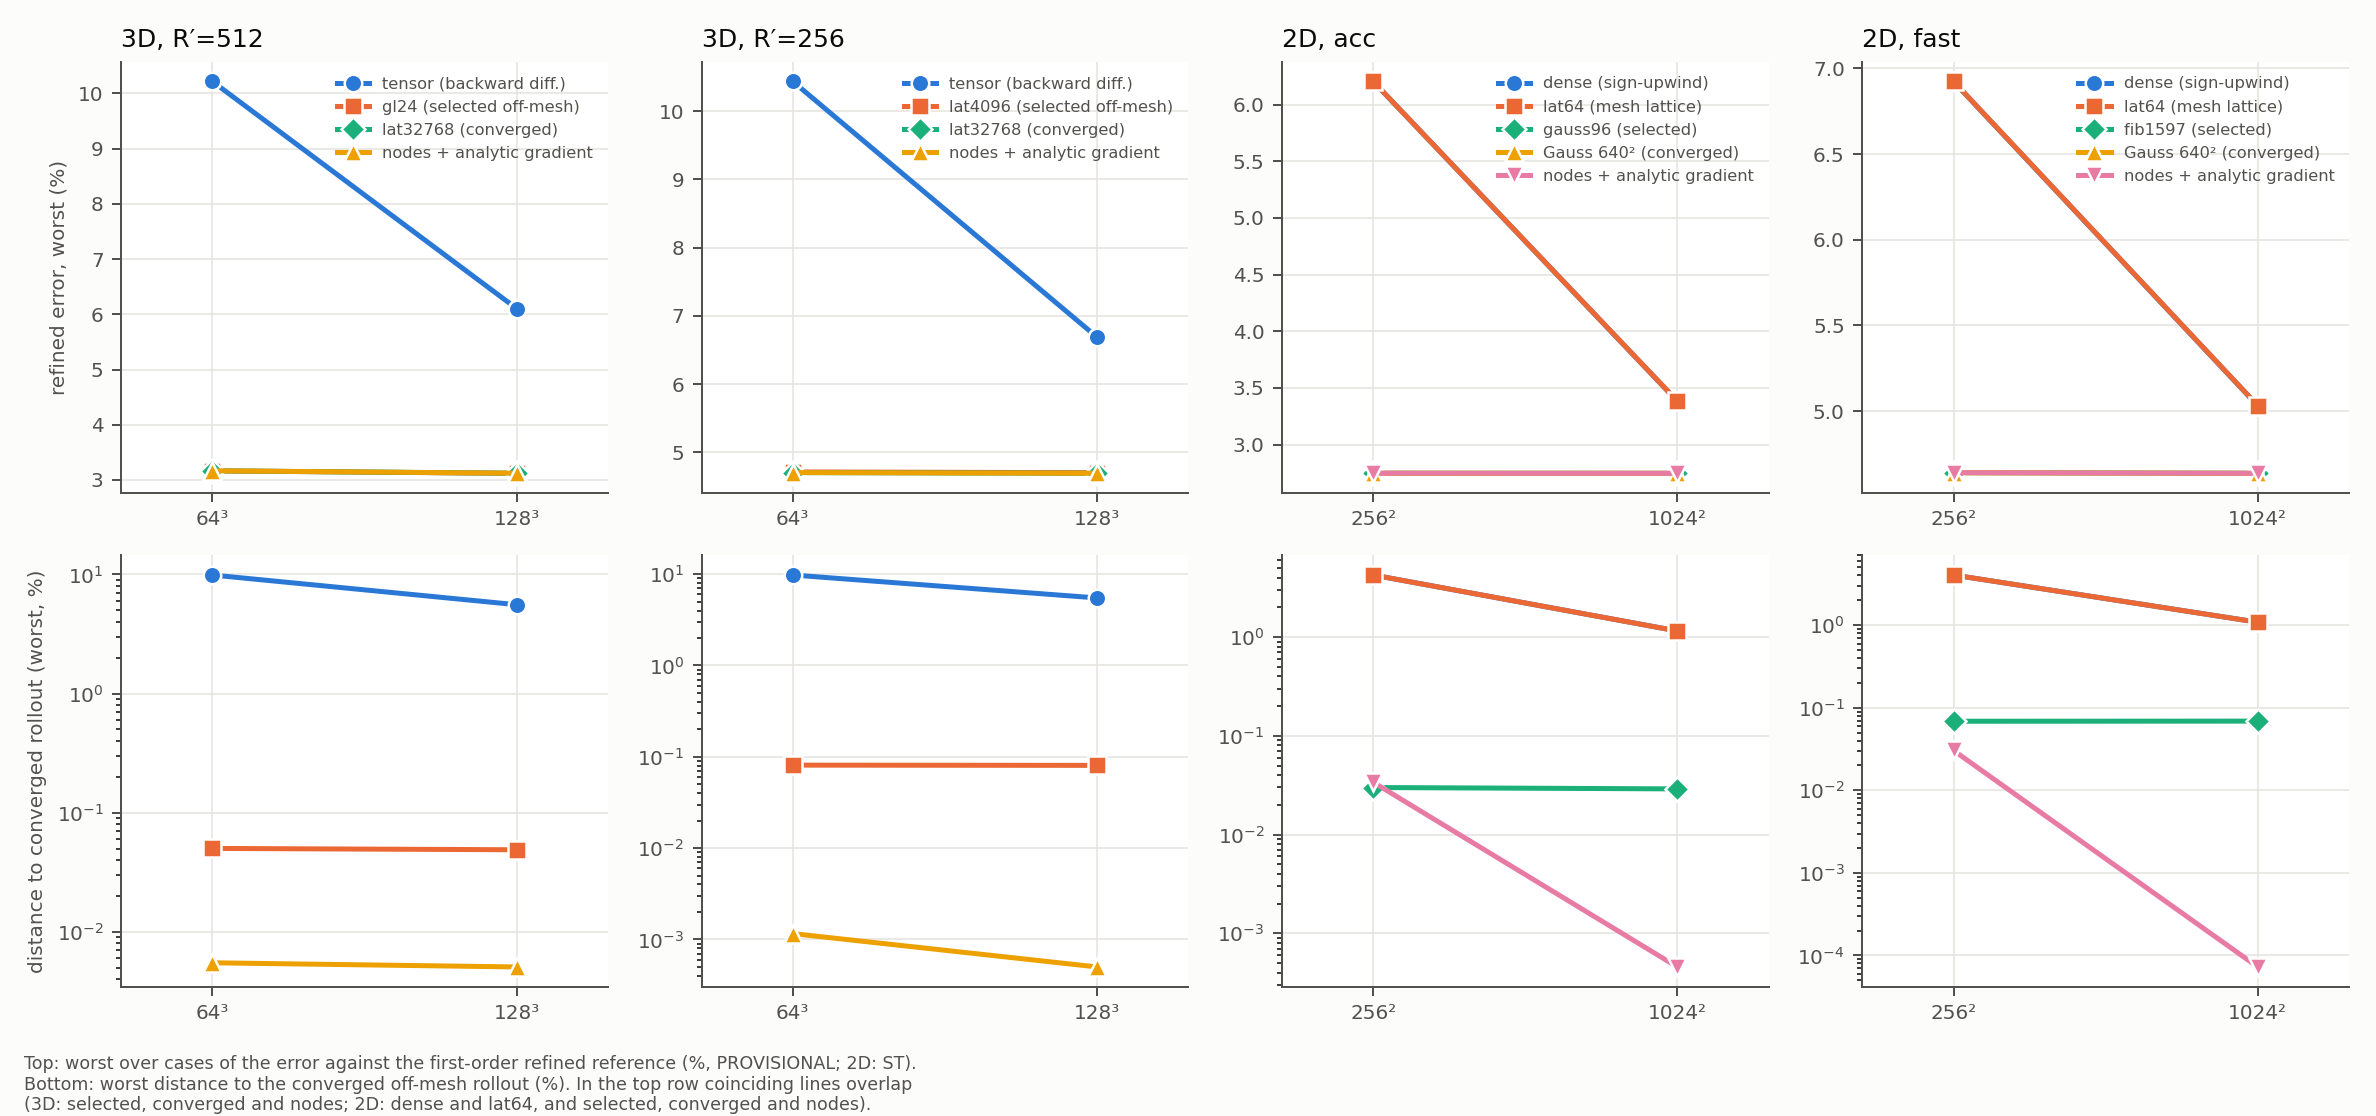
\includegraphics[width=\linewidth]{figs/a1_error_vs_mesh.png}\end{center}

\subsection*{A2: the stencil gap follows the stencil order}
On fixed saved states, the gap between the mesh sum and the continuum integral falls with slope 0.99--1.00 for the first-order upwind stencil and 2.00 for second-order central differences, inside the pre-registered bars in all four panels, with both controls behaving.
With the exact gradient the gap reaches the reference's noise floor, so its slope is not resolved.
\begin{center}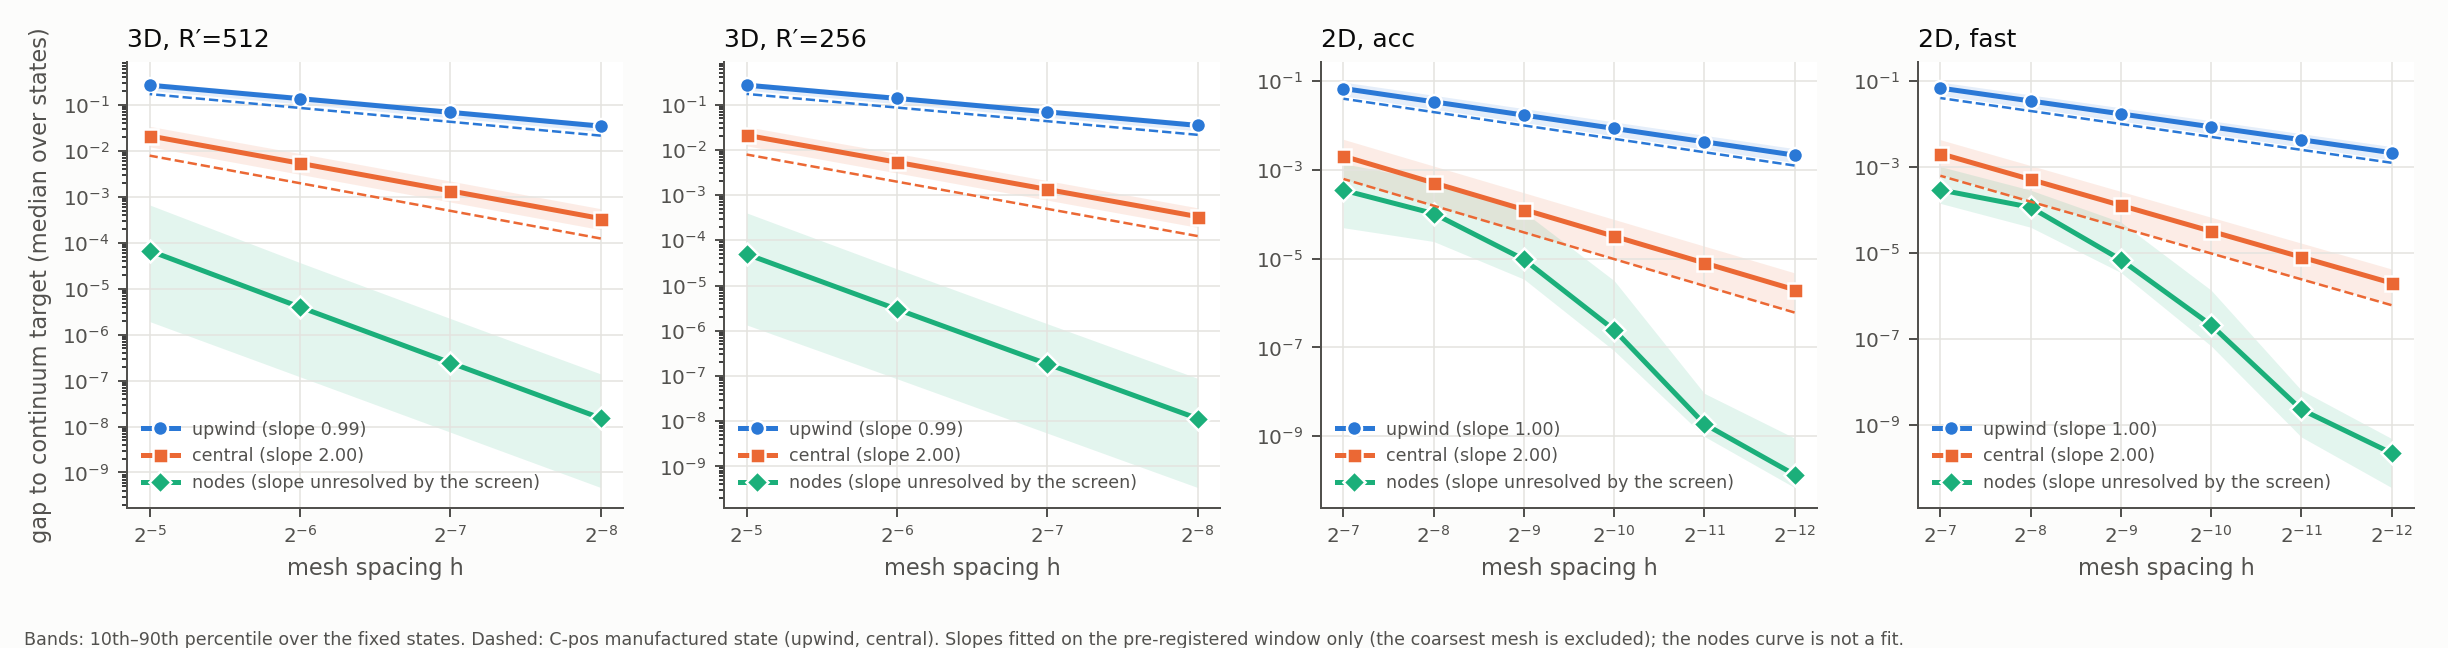
\includegraphics[width=\linewidth]{figs/a2_gap_vs_h.png}\end{center}

\subsection*{What this changes in the paper}
Kill criterion K1 fired in its useful form. The accuracy gain comes from evaluating the continuum term with the exact gradient, not from placing points off the mesh.
\begin{itemize}
\item The claim becomes: exact-gradient \emph{continuum evaluation} gives the accuracy.
\item Classical quadrature (thousands of points, independent of the mesh) gives it cheaply. The mesh-node arm needs every node: about $2.5\times10^5$ at 64\textsuperscript{3} and $2\times10^6$ at 128\textsuperscript{3}.
\end{itemize}

\subsection*{Changed or corrected along the way}
\begin{itemize}
\item The 2D finite-difference gradient gate was redesigned as a convergence check (the bank is steep near the walls; the analytic gradient is correct).
\item Historical cohort hashes are now report-only, because they include GPU floats.
\item A non-finite target now invalidates a result rather than being retried.
\item A halved A2 state set was caught by the code audit before the job ran.
\end{itemize}
Open: whether to pre-register a new 2D separation rule, and a solver-sensitivity rerun at 128\textsuperscript{3}. A3 and A4 remain deferred.
